\documentclass[25pt]{tikzposter}
\geometry{paperwidth=36in,paperheight=48in}

\usepackage[utf8]{inputenc}
\usepackage{tikz}

\usepackage[pangram]{blindtext}
\usepackage{comment}
\usetikzlibrary{arrows.meta}

\newcommand{\largearrow}{-{Latex[length=3mm,width=5mm]}}


\tikzset{%
  >={Latex[width=2mm,length=2mm]},
  % Specifications for style of nodes:
            base/.style = {rectangle, rounded corners, draw=black,
                           minimum width=8cm, minimum height=1cm,
                           text centered, font=\sffamily},
		startstyle/.style = {base, fill=blue!30},
		astyle/.style = {base, fill=red!30},
		bstyle/.style = {base, fill=green!30},
		cstyle/.style = {base, minimum width=2.5cm, fill=orange!15,
                           font=\ttfamily},
}

\usetheme{Rays}
\usecolorstyle[colorPalette=BrownBlueOrange]{Germany}

\title{Twitter Fire Scraper}
\author{Coding Team}
\date{\today}
\institute{Illinois Institute of Technology}

\begin{document}

\maketitle

\block{~}
{
    \blindtext
}

\begin{columns}
    \column{0.4}
    \block{More text}{Text and more text}
    
    \column{0.6}
    \block{Something else}{Here, \blindtext \vspace{4cm}}
    \note[
        targetoffsetx=-9cm, 
        targetoffsety=-6.5cm, 
        width=0.5\linewidth
        ]
        {e-mail \texttt{sharelatex@sharelatex.com}}
\end{columns}

\begin{columns}
    \column{0.5}
    \block{A figure}
    {
        \begin{tikzfigure}
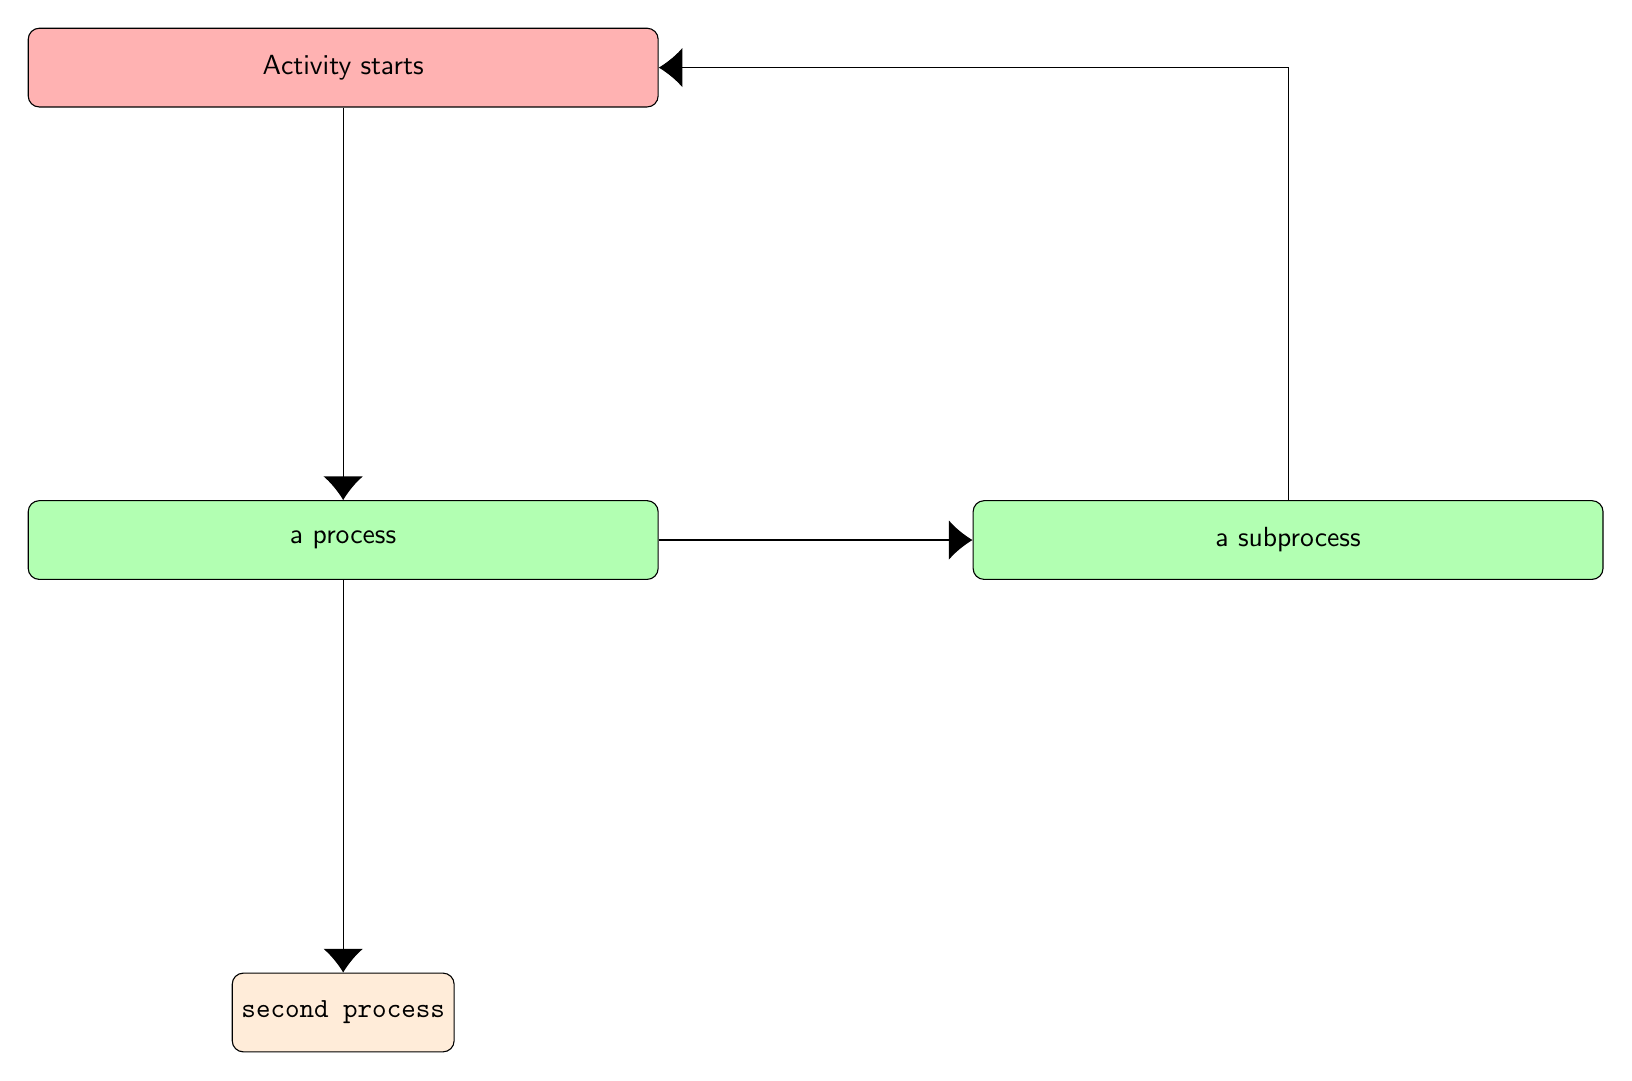
\begin{tikzpicture}[node distance=6cm,
    every node/.style={fill=white, font=\sffamily}, align=center]
  % Specification of nodes (position, etc.)
  \node (start)	[astyle]										{Activity starts};
  \node (a)		[bstyle, below of=start]				{a process};
  \node (asub)	[bstyle, right of=a, xshift=6cm]	{a subprocess};
  \node (b)		[cstyle, below of=a]						{second process};
  
  % Specification of lines between nodes specified above
  % with aditional nodes for description 
	\draw[\largearrow]	(start) -- 		(a);
	\draw[\largearrow]	(a) -- 				(b);
	\draw[\largearrow]	(a) -- 				(asub);
	\draw[\largearrow]	(asub) |- 			(start);
  \end{tikzpicture}
        \end{tikzfigure}
    }
    \column{0.5}
    
    \block{Description of the figure}{\blindtext}

\end{columns}

\begin{columns}

	\column{0.5}
	\block{a}
	{
		a first block
	}

	\column{0.5}
	\block{a}
	{
		a second block
	}
\end{columns}

\end{document}
